\documentclass[12pt, letterpaper]{article}
\usepackage[utf8]{inputenc}

\usepackage{amsmath,amssymb}
\usepackage{graphicx}
\usepackage{afterpage}
\usepackage{placeins}
\usepackage{caption}

\title{\vspace{-3cm} Take-Home Final}
\author{Wesley Giotta}
\date{\today}

\begin{document}
\maketitle

I started in Python3 and then finished in R. I found that all the urls were the same with the exception of the year, so I made a list of all the urls by adding the appropriate number to the year for the census and election urls.

After that I used BeautifulSoup and made functions to grab the needed table from a url and then looped through it for them all. Because the length for the election tables were not all the same I made the range for the loop very long but had it break when it hit the total at the bottom of the tables. Also, I had to make sure that the democrat and republican data went in the correct columns by having the function check if the first column had democratic or not. The census table was much nicer with the exception of the column for population sometimes swapping.

Then the nested lists that the functions gave me were insterted into a SQL database using sqlite3 and an index was made to make sure I did not insert the data twice by accident.

Lastly, I selected the asked for results and used Rstudio's ggplot2, dplyr, and RSQLite packages to make the graphs.\\

Results from the SQL select for the fraction of the 1980 population that voted for Ronald Regan (Republican).
\begingroup\makeatletter\def\@currenvir{verbatim}
\verbatim
state       Rfraction 
----------  ----------
Georgia     0.1197    
Hawaii      0.1349    
South Caro  0.1413    
North Caro  0.1556    
Maryland    0.1614    
Rhode Isla  0.1634    
New York    0.1648    
Alabama     0.168     
West Virgi  0.1714    
Tennessee   0.1716    
Kentucky    0.1735    
Mississipp  0.175     
Arkansas    0.1763    
Texas       0.1764    
Massachuse  0.1844    
Vermont     0.185     
Virginia    0.1851    
Delaware    0.1872    
Louisiana   0.1885    
Pennsylvan  0.1907    
California  0.1912    
New Mexico  0.1925    
Nevada      0.1937    
Arizona     0.1949    
Ohio        0.2044    
Illinois    0.2064    
Michigan    0.2068    
Washington  0.2094    
Florida     0.21      
New Jersey  0.21      
Maine       0.2121    
Minnesota   0.2142    
Oregon      0.2169    
Connecticu  0.2179    
Missouri    0.2185    
Colorado    0.2257    
Indiana     0.2287    
Oklahoma    0.2299    
Wisconsin   0.2314    
Iowa        0.232     
Wyoming     0.2358    
Kansas      0.2398    
New Hampsh  0.2408    
Montana     0.2629    
Nebraska    0.2675    
South Dako  0.2871    
North Dako  0.2968    
Utah        0.3009    
Idaho       0.308 
\end{verbatim}

\begin{figure}[!ht]
\textbf{1.}\par\medskip
\caption*{1976 Scatter plot of two-party shares of votes}
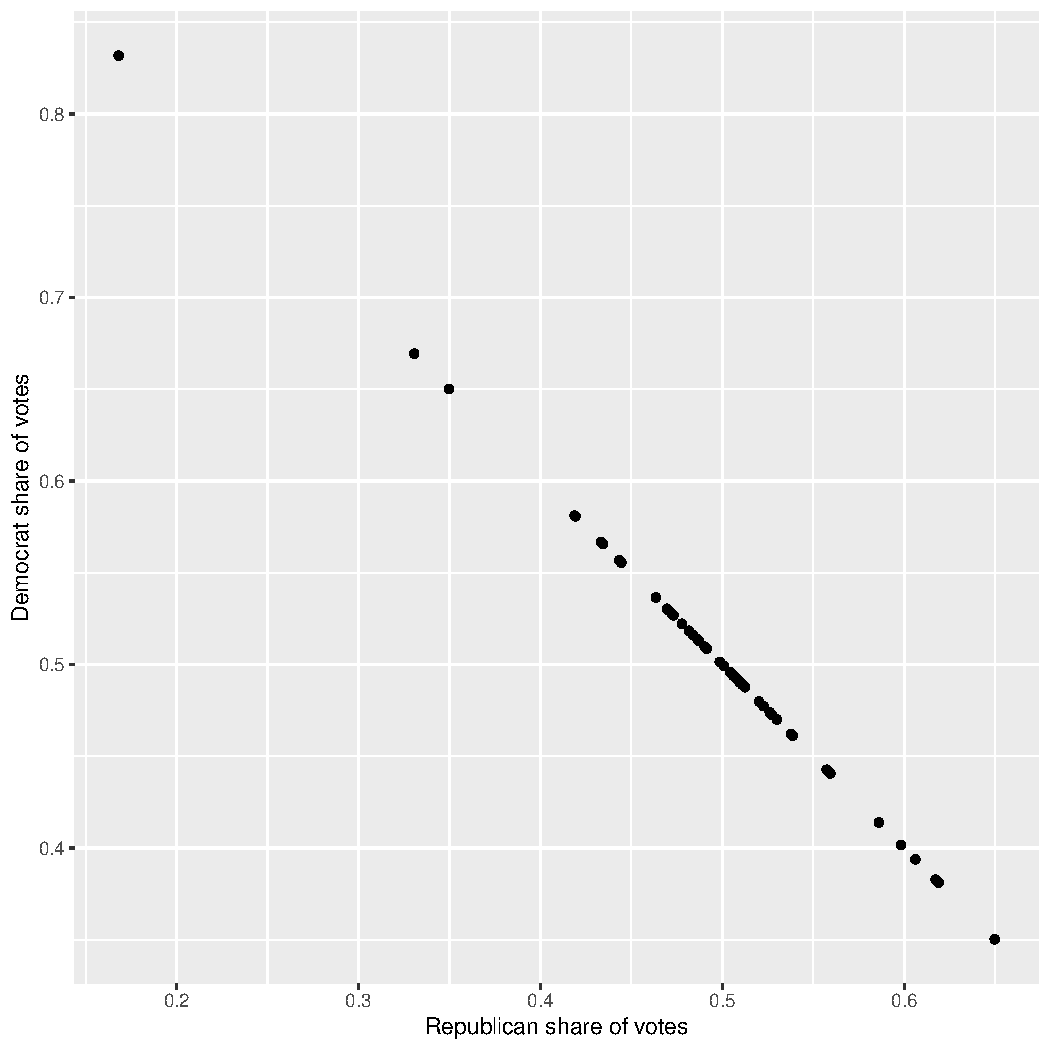
\includegraphics[scale=0.9]{shares_1.pdf}
\end{figure}

\begin{figure}[!ht]
\textbf{2. a)}\par\medskip
\caption*{1976 Cumulative distribution of electoral votes over vote-shares}
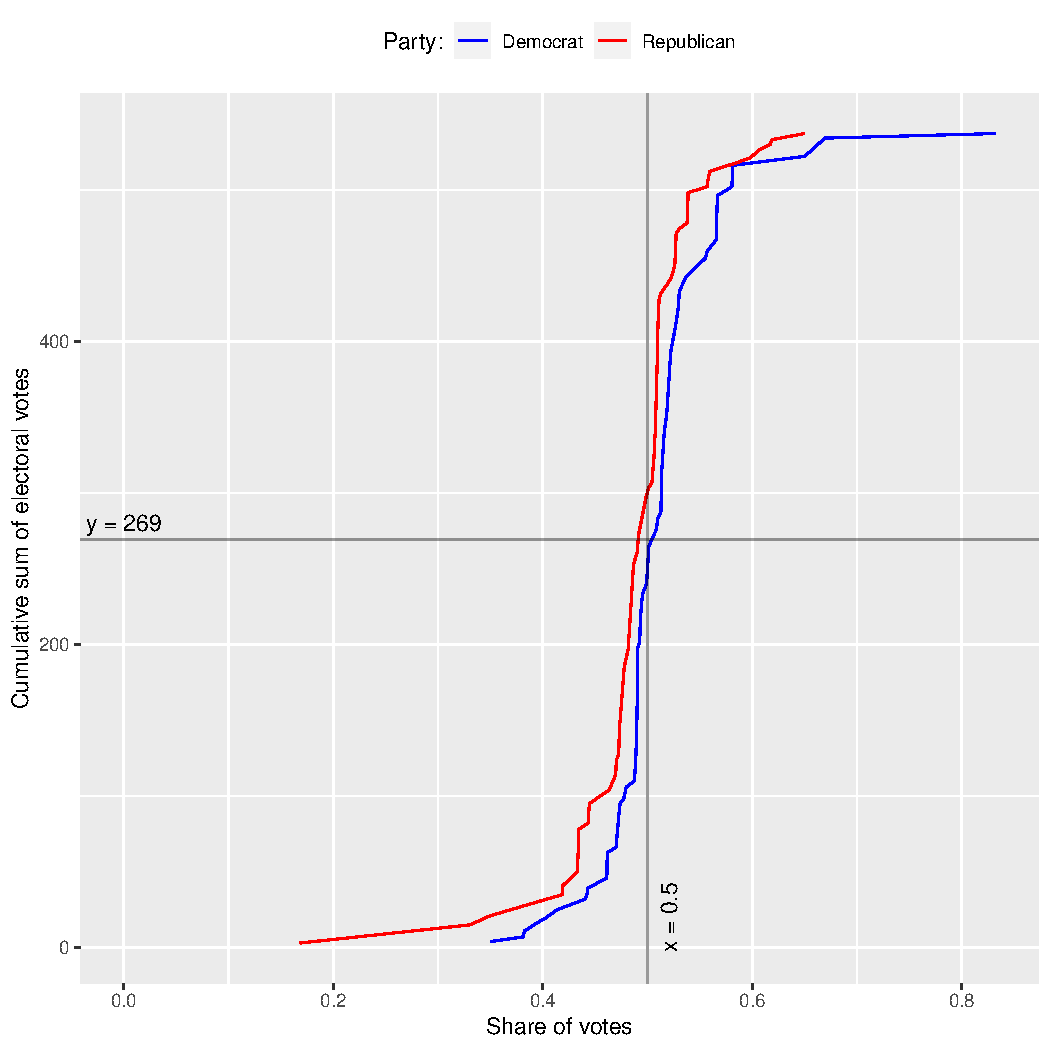
\includegraphics[scale=0.9]{cdf_2a.pdf}
\end{figure}

\begin{figure}[!ht]
\textbf{2. b)}\par\medskip
\caption*{2000 Cumulative distribution of electoral votes over vote-shares}
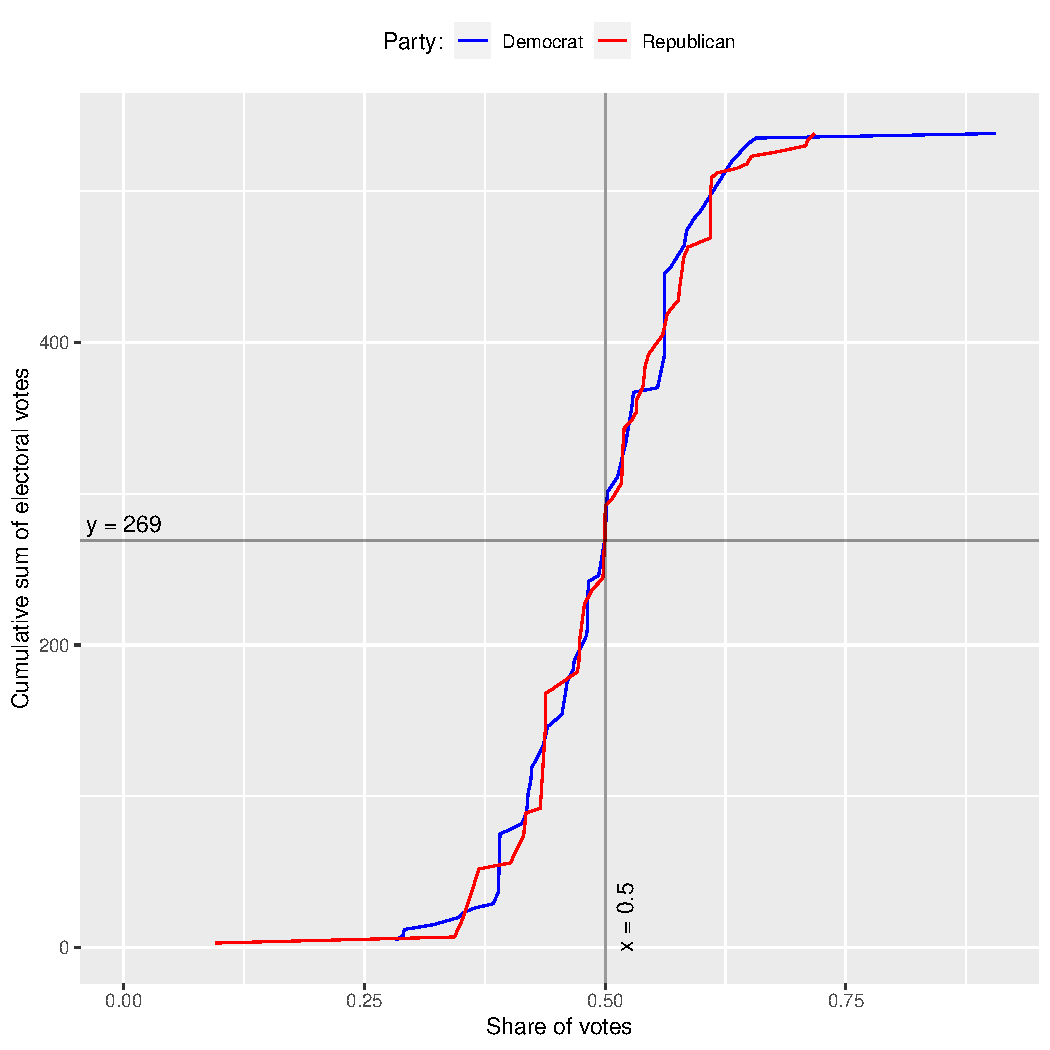
\includegraphics[scale=0.9]{cdf_2b.pdf}
\end{figure}

\begin{figure}[!ht]
\textbf{2. c)}\par\medskip
\caption*{2016 Cumulative distribution of electoral votes over vote-shares}
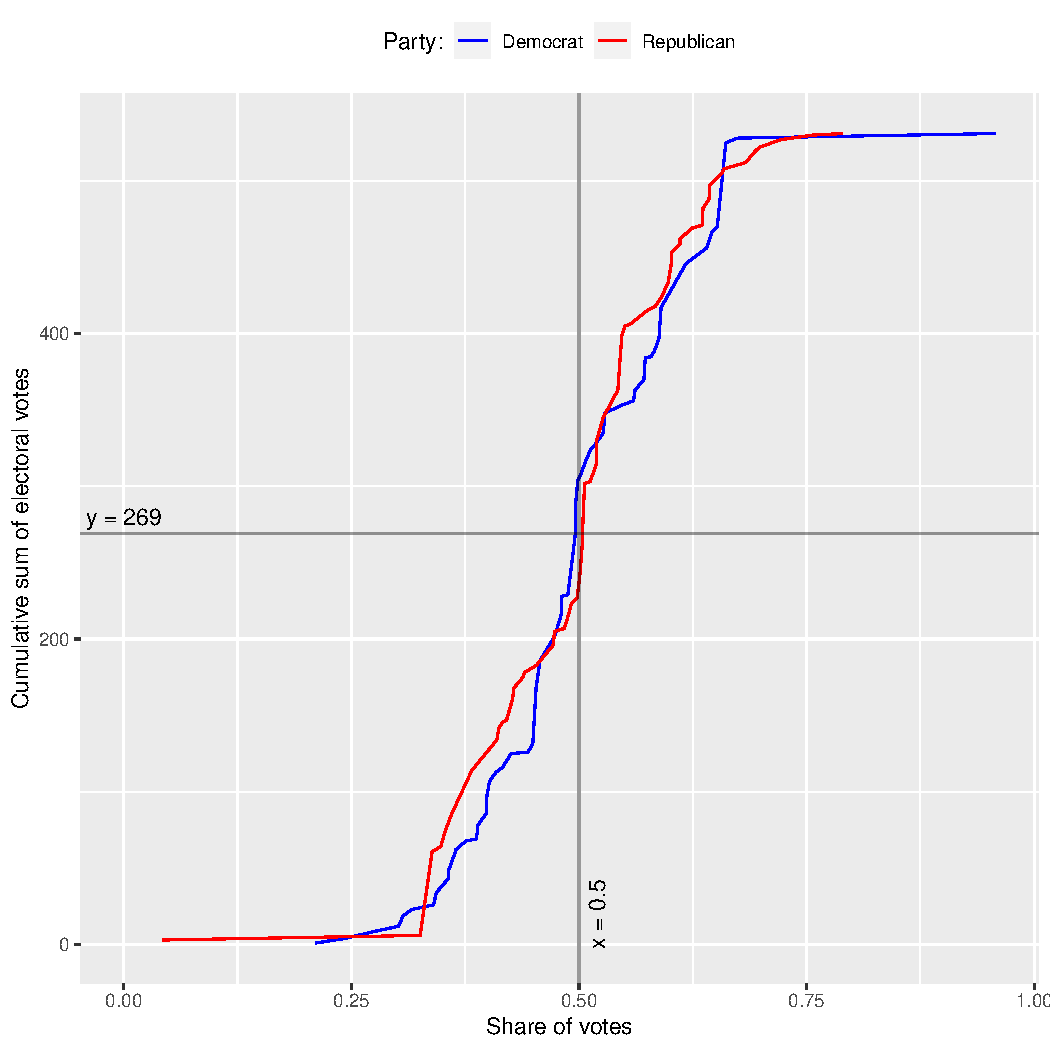
\includegraphics[scale=0.9]{cdf_2c.pdf}
\end{figure}



\end{document}
